\documentclass[
	12pt,				% tamanho da fonte
	openright,			% capítulos começam em pág ímpar (insere página vazia caso preciso)
	oneside,			% para impressão em recto e verso. Oposto a oneside
	a4paper,			% tamanho do papel. 
	english,			% idioma adicional para hifenização
	french,				% idioma adicional para hifenização
	spanish,			% idioma adicional para hifenização
	brazil				% o último idioma é o principal do documento
	]{abntex2}

\usepackage{lmodern}			% Usa a fonte Latin Modern			
\usepackage[T1]{fontenc}		% Selecao de codigos de fonte.
\usepackage[utf8]{inputenc}		% Codificacao do documento (conversão automática dos acentos)
\usepackage{indentfirst}		% Indenta o primeiro parágrafo de cada seção.
\usepackage{color}				% Controle das cores
\usepackage{graphicx}			% Inclusão de gráficos
\usepackage{microtype} 			% para melhorias de justificação
\usepackage{transparent}
\usepackage{eso-pic}
\usepackage{amsthm,amsfonts}
\usepackage{float}
\usepackage{multirow}
\usepackage[table,xcdraw]{xcolor}
\usepackage{longtable}
\usepackage{lipsum}				% para geração de dummy text
%\usepackage[brazilian,hyperpageref]{backref}	 % Paginas com as citações na bibl
\usepackage[alf]{abntex2cite}	% Citações padrão ABNT
\usepackage{xcolor}
\usepackage{scalefnt}

\usepackage[font=small]{caption}     %% make caption in normal size
\usepackage{etoolbox}
\AtBeginEnvironment{longtabu}{\footnotesize}{}{}   %% change all longtabu content to foot note size

\definecolor{verde}{rgb}{0,0.5,0}
\usepackage{listings}
\lstset{
  language=C++,
  basicstyle=\ttfamily\small,
  keywordstyle=\color{blue},
  stringstyle=\color{verde},
  commentstyle=\color{red},
  extendedchars=true,
  showspaces=false,
  showstringspaces=false,
  numbers=left,
  numberstyle=\tiny,
  breaklines=true,
  backgroundcolor=\color{green!10},
  breakautoindent=true,
  captionpos=b,
  xleftmargin=0pt,
}


\titulo{Estudo Sobre o Processamento do Milho}
\autor{Gabriel Rodrigues Munhoz 106802\\João Vítor Batistão 108074}
\local{Maringá, PR}
\data{09.10.2022}
\orientador{}
\coorientador{}
\instituicao{%
  Universidade Estadual de Maringá - UEM
  \par
  Departamento de Engenharia de Produção - DEP}
\tipotrabalho{Tese (Doutorado)}
\preambulo{}

\definecolor{blue}{RGB}{41,5,195}

\makeatletter
\hypersetup{
     	%pagebackref=true,
	pdftitle={\@title}, 
	pdfauthor={\@author},
    	pdfsubject={\imprimirpreambulo},
	pdfcreator={LaTeX with abnTeX2},
	pdfkeywords={abnt}{latex}{abntex}{abntex2}{trabalho acadêmico}, 
	colorlinks=true,       		% false: boxed links; true: colored links
    	linkcolor=black,          	% color of internal links
    	citecolor=black,        		% color of links to bibliography
    	filecolor=magenta,      		% color of file links
	urlcolor=blue,
	bookmarksdepth=4
}

\setlength{\parindent}{1.3cm}

\setlength{\parskip}{0.2cm}  % tente também \onelineskip

\makeindex

%\usepackage{fancyhdr}
%\fancyhead{}
%\fancyfoot{}
%\lhead{Processo Agroindustrial de Processamento de Cacau}
%\rhead{Processo Agroindustrial de Processamento de Cacau}

\AddToShipoutPicture{
\put(0,0){
\parbox[b][\paperheight]{\paperwidth}{%
\vfill
\centering
{\transparent{0.1}\includegraphics[scale=1.4]{../../Pictures/logoUEM.jpg}    }%
\vfill}}}



%\graphicspath{{../Pictures}}
\begin{document}

\begin{minipage}[c][0cm][c]{0cm} % a primeira minipágina tem uma altura de 1.5cm e uma largura de 3cm.

\centering


\includegraphics[scale=0.45]{../../Pictures/uem-modelo-04.png}  
\end{minipage}

\selectlanguage{brazil}

\frenchspacing 

% \pretextual

\imprimircapa


% ---
% RESUMOS
% ---

%\setlength{\absparsep}{18pt} % ajusta o espaçamento dos parágrafos do resumo
%\begin{resumo}
 
 
% \textbf{Palavras-chave}: latex. abntex. editoração de texto.
%\end{resumo}


% ---
% inserir o sumario
% ---
\pdfbookmark[0]{\contentsname}{toc}
\tableofcontents*
\cleardoublepage

% ----------------------------------------------------------
% ELEMENTOS TEXTUAIS
% ----------------------------------------------------------
\textual

\chapter{Introdução}
%\pagestyle{fancy}

O milho é um cereal comum no Brasil, muito utilizado para alimentação, tanto \textit{in natura} como processado, e é também muito utilizado para fabricação de óleos e outros derivados tanto para a população em geral, quanto para a indústria. Essa versatilidade do grão vem da sua composição, rica em amido, proteínas, óleo e fibras; e também dos diferentes tipos de milho existentes. Na imagem \ref{1} é possível verificar os diversos produtos obtidos com base em grãos secos de milho, milho verde e milho doce.

\begin{figure}[H]
\begin{center}
\caption{Produtos obtidos do milho}
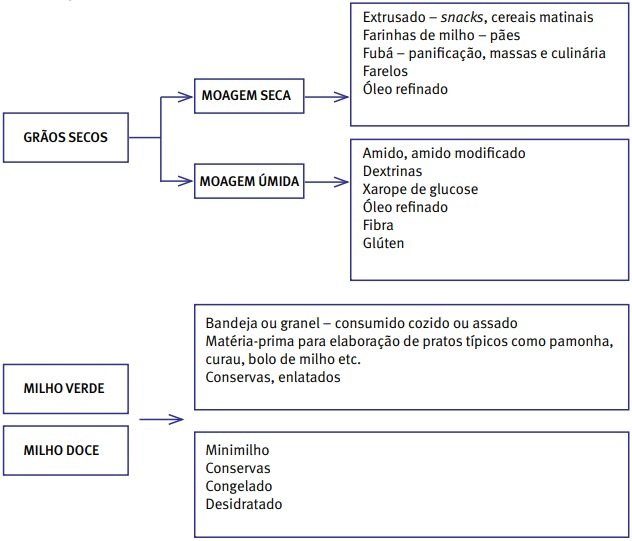
\includegraphics[scale=0.5]{Imagens/WhatsApp Image 2022-10-09 at 14.40.21.jpeg} 
\legend{Fonte: \cite{regitano2015processamento}}
\label{1}
\end{center}
\end{figure}

O grão de milho é composto basicamente de 3 partes: endosperma, pericarpo e germe. O endosperma é rico em amido e representa a maior parte do grão, o germe ou gérmen é rico em óleo e o pericarpo é a casca do milho que é muito rica em fibras. Cada uma dessas partes é utilizada para a produção de um tipo especíifico de produto. \cite{paes2006aspectos}

\begin{figure}[H]
\begin{center}
\caption{Composição básica do grão do milho}
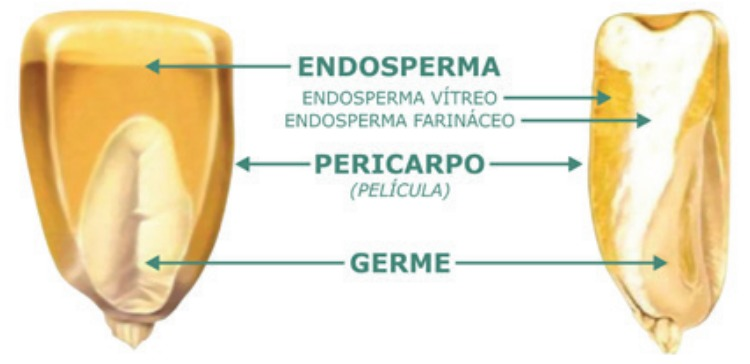
\includegraphics[scale=0.4]{Imagens/WhatsApp Image 2022-10-09 at 14.56.22.jpeg} 
\legend{Fonte: Associação Brasileira das Indústrias do Milho (Abimilho)}
\end{center}
\end{figure}

Para obter esses diferentes derivados do mesmo produto a indústria precisou desenvolver 2 diferentes fluxos de processamento, o de via úmida e o de via seca. O de via seca é um processo mais antigo e tem como base a quebra física do grão de milho de forma com que a umidade não ultrapasse 20$\%$. Nesse fluxograma o germe é retirado inicialmente e a moagem se estende por mais ou menos tempo de acordo com o subproduto que a indústria deseja obter. \cite{strazzi2015derivados}

\begin{figure}[H]
\begin{center}
\caption{Fluxograma de processamento do milho por via seca}
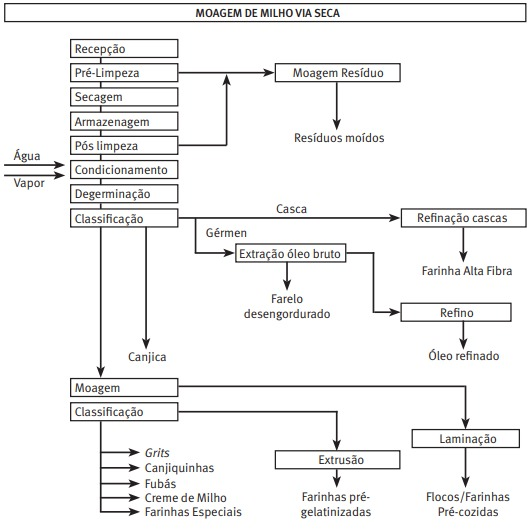
\includegraphics[scale=0.55]{Imagens/WhatsApp Image 2022-10-09 at 14.41.23.jpeg} 
\legend{Fonte: \cite{strazzi2015derivados}}
\end{center}
\end{figure}

No processo de via úmida, diferentemente do anterior, há um alto teor de umidade e também a ocorrência de fermentação. O grão primeiramente é macerado por um período de 36 a 48 horas em contato com água e dióxido de enxofre a 50ºC - 54ºC para fermentação. Somente após esse processo que é realizada a separação do germe para a utilização do mesmo para a produção do óleo de milho. E em seguida, são realizadas diversas outras etapas para separação de fibras, glúten, dextrinas e principalmente retirada da água, como é possível verificar na imagem \ref{2}. \cite{strazzi2015derivados}

\begin{figure}[H]
\begin{center}
\caption{Fluxograma de processamento do milho por via úmida}
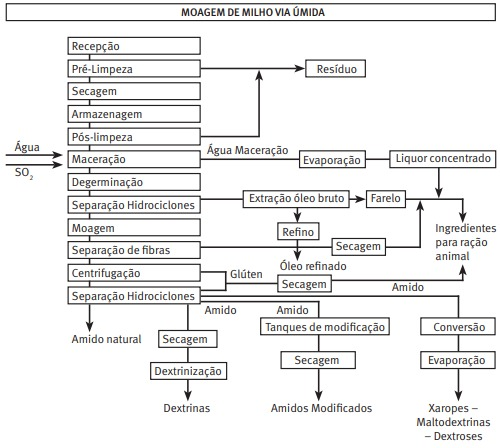
\includegraphics[scale=0.55]{Imagens/WhatsApp Image 2022-10-09 at 14.41.43.jpeg} 
\legend{Fonte: \cite{strazzi2015derivados}}
\label{2}
\end{center}
\end{figure}

%\newpage
\chapter{Processamento}
%\pagestyle{fancy}
\section{Amido de Milho}


\begin{figure}[H]
\begin{center}
\caption{Fluxograma do processo de produção de amido de milho}
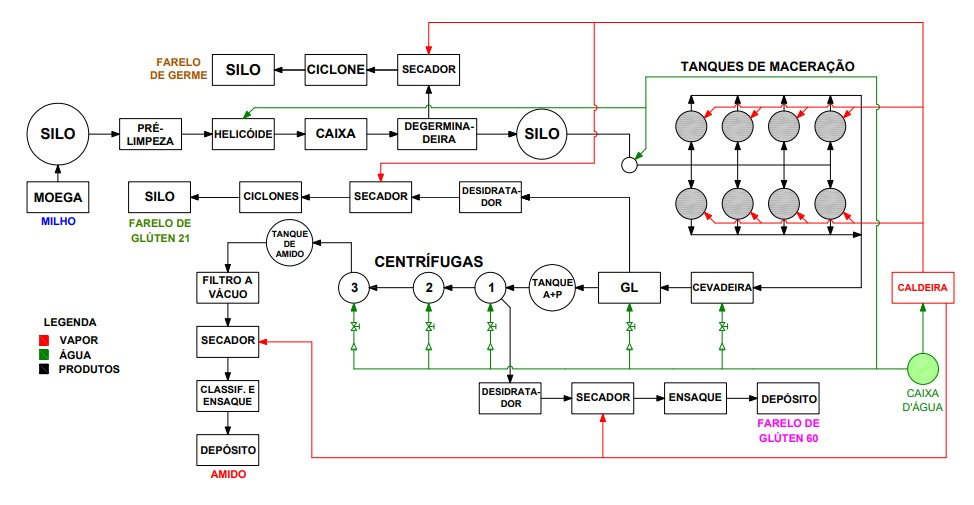
\includegraphics[scale=0.4]{Imagens/WhatsApp Image 2022-10-09 at 14.21.26.jpeg} 
\legend{Fonte: \cite{da2019analise}}
\end{center}
\end{figure}


O processamento do milho para produção de amido é realizado por via úmida, uma das maneiras de processar o produto. Desse modo, a primeira etapa é composta pela retirada de impurezas por meio de peneiras, sopradores, separadores magnéticos entre outros maquinários. Após a limpeza inicial os grãos são transportados para maceradores onde recebem água (50ºC - 55ºC) e dióxido de enxofre, e são triturados e sofrem fermentação lática. Nesses tanques, os grãos macerados são processados por até 48 horas, isso faz com que os grãos se tornem mais macios, limitem a ação de microorganismos e atinjam 50$\%$ de umidade, é a fase mais importante do processamento de via úmida. \cite{da2019analise}

A maceração pode ser subdividida em 3 fases, sendo a primeira caracterizada pela hidratação e fermentação lática do milho, a segunda pela penetração do dióxido de enxofre no interior do grão e a terceira fase pela hidrólise das ligações nas proteínas do endosperma. Durante todas essas fases é necessário um controle rígido da temperatura, pois ela deve ser mantida acima de 47ºC e abaixo de 53ºC para que a fermentação lática ocorra com qualidade e não apareçam leveduras produtoras de álcool. \cite{peixoto2017avaliaccao}

Em seguida, os grãos seguem para moinhos de discos e após a moagem é realizada a separação dos germes que são destinados para a indústria de óleos. O germe é mais leve que o endosperma e a película do milho, então é facilmente separado na máquina chamada de degerminadeira por meio de força centrífuga. \cite{geraldi2010estudo}

O material sem os germes é novamente moído e separado da fibra, por meio de peneiras e centrífugas, e por fim é retirado também o glúten através de centrífugas verticais de alta rotação, restando apenas o amido úmido. E a última etapa é representada pela filtração e secagem para que o amido final atinja a marca de no máximo 14$\%$ de umidade, obedecendo assim a legislação brasileira e podendo ser comercializado normalmente. \cite{da2019analise}


\section{Conserva de Minimilho}

Antes de realizar a descrição do processo produtivo do minimilho, é importante se entender sobre a matéria prima em si. O minimilho na verdade é a inflorescência feminina do milho, contendo valor calórico semelhante a alguns vegetais. 

Para a comercialização, é passível de acontecer com palha ou sem palha, sendo de extrema importância para o consumidor final a aparência do produto, englobando coloração, , forma, comprimento e diâmetro. Para toda a produção até a chegada no consumidor final, o adequado para o minimilho é que sejam aplicadas as boas práticas de fabricação (BPFs) em todos os subprocessos, como mostrado a seguir:


\begin{figure}[H]
\begin{center}
\caption{Fluxograma do processo de produção de conserva de minimilho}
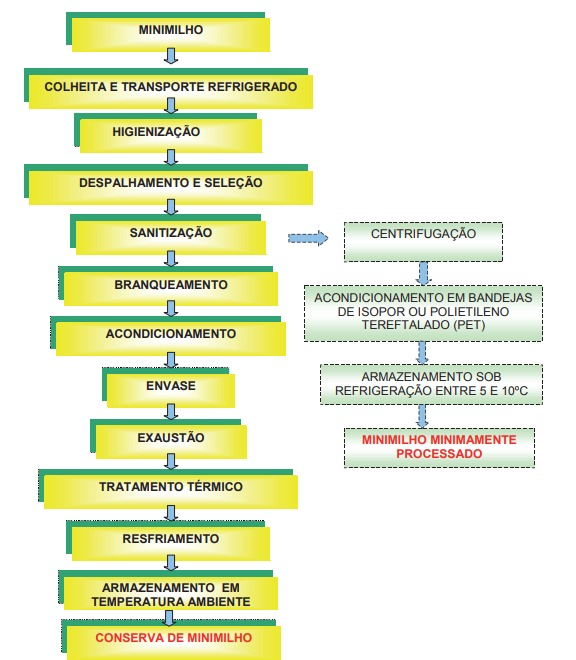
\includegraphics[scale=0.4]{Imagens/WhatsApp Image 2022-10-09 at 14.25.06.jpeg} 
\legend{Fonte: \cite{queiroz2010processo}}
\end{center}
\end{figure}

Quanto ao processo de produção do minimilho, este se inicia na colheita e no transporte da matéria prima, no qual a primeira deve acontecer de forma estritamente manuel e nos primeiros momentos da manhã, sendo colhidas prioritariamente com palha. Já quanto à logística, deve ocorrer em um veículo minimamente refrigerado, a fim de conservar as principais características do produto.

Uma vez o minimilho chegado ao destino intermediário como por exemplo a indústria, deve acontecer a higienização, pré-lavagem, despalhamento, seleção e sanitização, a fim de tornar possível os próximos passos do processo produtivo. Para a higienização e pré lavagem, deve acontecer com água potável em um primeiro momento, antes mesmo de acontecer o despalhamento, após isso é importante acontecer a imersão dessas espigas em solução aquosa de cloro. O próximo passo é o despalhamento e seleção, ambos autoexplicativos. Em seguida, a sanitização acontece em submersão assim como na higienização, no entanto agora em solução aquosa de hipoclorito de sódio a 20$\%$. \cite{queiroz2010processo}
	
	Com a finalização da sanitização se faz necessário o branqueamento, processo que inativa enzimas indesejáveis, que acontece a partir do milho dentro de recipiente com água fervente totalmente imersos por 2 minutos e em seguida deve acontecer a imersão em água fria.
	
	Com isso, é importante acontecer o processo de exaustão, que visa eliminar o ar contido no interior do frasco, com o objetivo de formar vácuo. A temperatura da solução deve ser de 85 a 87 graus celsius e entre 15 e 20 minutos, e assim os frascos devem ser imediatamente fechados, criando o vácuo. \cite{queiroz2010processo}
	
	O próximo passo é realizar o tratamento térmico ou a pasteurização, uma das etapas mais importantes por ter o objetivo de eliminar microrganismos que causam alterações nos alimentos e promover o cozimento das hortaliças.
	
	Em seguida acontece o resfriamento, que deve ser feito de forma imediata até a temperatura do sistema baixar para 40ºC.
Por fim acontece o armazenamento, que normalmente é feito por vidros, e deixados em locais escuros, secos e com boa ventilação e pode ficar armazenado por até 180 dias. \cite{queiroz2010processo}


\section{Xarope de Milho}

O xarope de glicose é um produto da hidrólise do amido, consistindo de monômeros e dímeros, oligossacarídeos e polissacarídeos.
Os xaropes são utilizados normalmente como adoçantes e componentes de meios de cultura para processos fermentativos.

\begin{figure}[H]
\begin{center}
\caption{Etapas do processamento enzimático do amido}
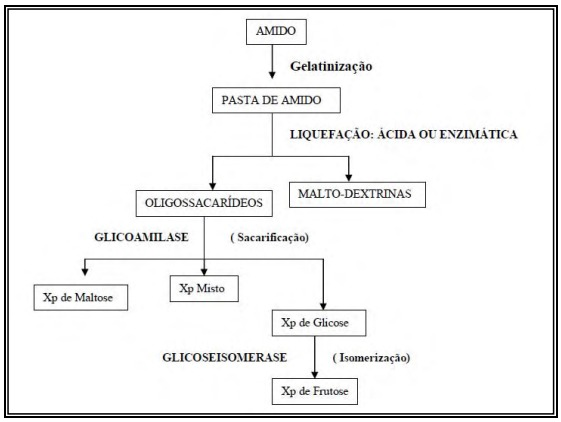
\includegraphics[scale=0.5]{Imagens/WhatsApp Image 2022-10-09 at 18.37.06.jpeg} 
\legend{Fonte: \cite{freitas2012desenvolvimento}}
\end{center}
\end{figure}

A produção em si do xarope consiste na hidrólise intensa do amido e acontece da seguinte forma: o amido é gelatinizado, se transformando e pasta de amido, em seguida acontece a liquefação ácida ou enzimática obtendo dois subprodutos: Oligossacarídeos e Malto-dextrinas, no qual os oligossacarídeos serão utilizados. Em seguida os oligossacarídeos são sacrificados a partir da glicoamilase chegando na Xp de maltose, Xp Misto e Xp de glicose, subproduto que será isomerizado a partir da glicose isomerase chegando no nosso objetivo o produto final, a Xp de Frutose.\cite{freitas2012desenvolvimento}


A partir da hidrólise do amido, os seguintes produtos são produzidos, na tabela abaixo além dos subprodutos, encontra-se suas aplicações:

\begin{figure}[H]
\begin{center}
\caption{Produtos provenientes da hidrólise do amido e suas aplicações}
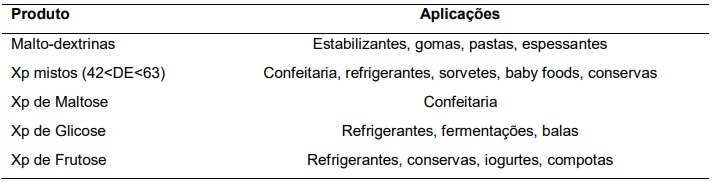
\includegraphics[scale=0.5]{Imagens/WhatsApp Image 2022-10-09 at 18.37.25.jpeg} 
\legend{Fonte: \cite{freitas2012desenvolvimento}}
\end{center}
\end{figure}

Na imagem é possível verificar os produtos provenientes da hidrólise do amido e suas aplicações.
Além disso, no Brasil o principal produto hidrolisado é um xarope específico, o DE 38-42. Já nos US, 50$\%$ da produção é distribuída para setores de balas, caramelos, padarias e confeitarias. 


%\newpage
\chapter{Conclusão}
%\pagestyle{fancy}

O milho é um produto muito versátil que pode ser comercializado desde in natura até ultraprocessado. Além de gerar inúmeros derivados ele também serve de base para muitos produtos alimentícios. Essa versatilidade advém de diferentes espécies de grãos e diferentes tipos de processos de beneficiamento. Neste trabalho foram descritos os 2 diferentes estilos de processamentos, o de via úmida e o de via seca, cada um produz uma variedade de produtos e possui uma tecnologia agregada diferente.

Um dos derivados mais importantes do milho é o amido de milho já que ele possui ampla utilização na área alimentícia, mas também é muito utilizado em diversos outros setores industriais. 

Produtos mais recentes como minimilho e o xarope de milho estão cada vez mais ganhando espaço no mercado. Além deles, outros produtos vão sendo criados e também mais aplicações vão sendo descobertas para os derivados já existentes.



\newpage
\postextual

\bibliography{referencias}

%\begin{anexosenv}

%\chapter{Código utilizado no software EMSO}

%\begin{lstlisting}
%\end{lstlisting}

%\end{anexosenv}

\end{document}